% docs/latex/groth-process.tex
\documentclass{standalone}
\usepackage{tikz}
\usetikzlibrary{arrows.meta,backgrounds,calc}

\begin{document}
	\pagecolor{white}
	\color{black}
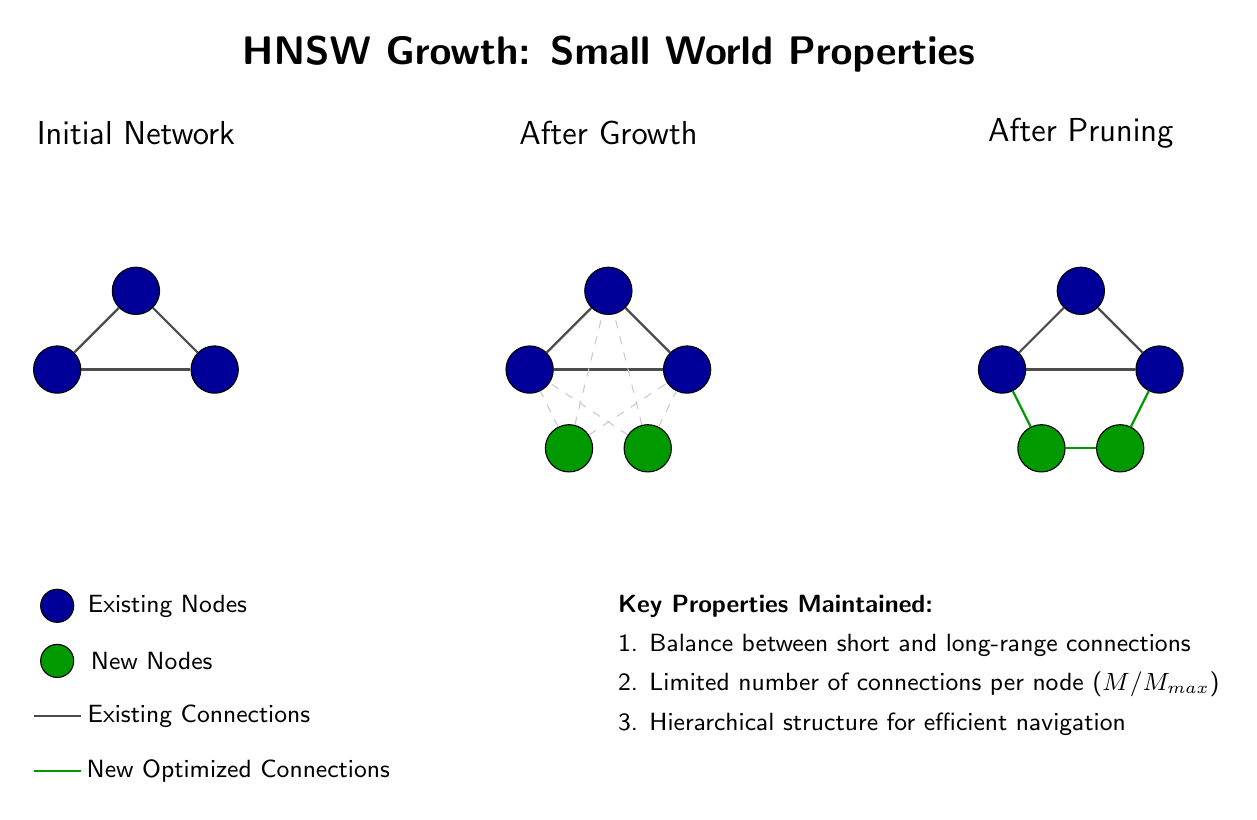
\begin{tikzpicture}[
    node/.style={circle, draw, fill=#1, minimum size=0.6cm},
    existing node/.style={node=blue!60!black},
    new node/.style={node=green!60!black},
    connection/.style={-, thick, gray!60!black},
    temp connection/.style={-, gray!40, dashed},
    new connection/.style={-, thick, green!60!black},
    stage label/.style={font=\sffamily\large},
    point label/.style={font=\small\sffamily}
]

% Title
\node[font=\Large\sffamily\bfseries] at (1,4) {HNSW Growth: Small World Properties};

% Stage Labels
\node[stage label] at (-5,3) {Initial Network};
\node[stage label] at (1,3) {After Growth};
\node[stage label] at (7,3) {After Pruning};

% Initial Network
\begin{scope}[shift={(-6,0)}]
    \node[existing node] (A1) at (0,0) {};
    \node[existing node] (B1) at (1,1) {};
    \node[existing node] (C1) at (2,0) {};
    \draw[connection] (A1) -- (B1);
    \draw[connection] (B1) -- (C1);
    \draw[connection] (A1) -- (C1);
\end{scope}

% Growth Phase
\begin{scope}
    \node[existing node] (A2) at (0,0) {};
    \node[existing node] (B2) at (1,1) {};
    \node[existing node] (C2) at (2,0) {};
    \node[new node] (D2) at (0.5,-1) {};
    \node[new node] (E2) at (1.5,-1) {};
    
    \draw[connection] (A2) -- (B2);
    \draw[connection] (B2) -- (C2);
    \draw[connection] (A2) -- (C2);
    
    \draw[temp connection] (D2) -- (A2);
    \draw[temp connection] (D2) -- (B2);
    \draw[temp connection] (D2) -- (C2);
    \draw[temp connection] (E2) -- (A2);
    \draw[temp connection] (E2) -- (B2);
    \draw[temp connection] (E2) -- (C2);
\end{scope}

% After Pruning
\begin{scope}[shift={(6,0)}]
    \node[existing node] (A3) at (0,0) {};
    \node[existing node] (B3) at (1,1) {};
    \node[existing node] (C3) at (2,0) {};
    \node[new node] (D3) at (0.5,-1) {};
    \node[new node] (E3) at (1.5,-1) {};
    
    \draw[connection] (A3) -- (B3);
    \draw[connection] (B3) -- (C3);
    \draw[connection] (A3) -- (C3);
    
    \draw[new connection] (D3) -- (A3);
    \draw[new connection] (D3) -- (E3);
    \draw[new connection] (E3) -- (C3);
\end{scope}

% Legend
\begin{scope}[shift={(-6,-3)}]
    \node[existing node, scale=0.7] (L1) at (0,0) {};
    \node[font=\small\sffamily] at (1.4,0) {Existing Nodes};
    
    \node[new node, scale=0.7] (L2) at (0,-0.7) {};
    \node[font=\small\sffamily] at (1.2,-0.7) {New Nodes};
    
    \draw[connection] (-0.3,-1.4) -- (0.3,-1.4);
    \node[font=\small\sffamily] at (1.8, -1.4) {Existing Connections};
    
    \draw[new connection] (-0.3,-2.1) -- (0.3,-2.1);
    \node[font=\small\sffamily] at (2.3,-2.1) {New Optimized Connections};
\end{scope}

% Key Points
\begin{scope}[shift={(1,-3)}]
    \node[font=\small\sffamily\bfseries, anchor=west] at (0,0) {Key Properties Maintained:};
    \node[font=\small\sffamily, anchor=west] at (0,-0.5) {1. Balance between short and long-range connections};
    \node[font=\small\sffamily, anchor=west] at (0,-1) {2. Limited number of connections per node ($M$/$M_{max}$)};
    \node[font=\small\sffamily, anchor=west] at (0,-1.5) {3. Hierarchical structure for efficient navigation};
\end{scope}

\end{tikzpicture}
\end{document}